\documentclass[12pt, letterpaper]{article}
\usepackage[a4paper, margin=1in]{geometry}
\usepackage{amsmath}
\usepackage{graphicx}
\usepackage{float}
\graphicspath{{images/}}
\author{Joseph Yu}
\title{Lab 3: Biologically Plausible Learning Rules in the Brain}
\begin{document}
\maketitle
\setcounter{section}{3}
\subsection{Oja's rule and Principal Component Analysis}
Oja's rule is based on the Hebbian learning rule but with a normalization term. From Hebbian learning we get the update rule for the weight vector is $\mathbf{\Delta w_i = \alpha x_i y} $ which updates the weight vector based on the alignment between the input and the output following the idea that "cells that fire together wire together". Oja's rule adds a normalization term to the update rule to prevent the weight vector from growing indefinitely. The update rule for Oja's rule is $\mathbf{\Delta w_i = \alpha (x_i y - y^2 w_i)}$. We can also derive from this update rule that the weight vector converges to the first principal component of the input data.
\[ \Delta w = \alpha (x y - y^2 w) \]
\[ \Delta w = \alpha (x x^T w - w^T x x^T w w) \]
\[ \Delta w = \alpha (C w - w^T C w w) \] where $\mathbf{C = x x^T}$ is the covariance matrix of the input data. 
We can see that once the weight vector converges, $\mathbf{C w = w^T C w w}$ and we get that $w$ is an eigenvector of $C$ when $ \| \mathbf{w} \|_2 = 1$. Further proofs actually demonstrate that the weight vector converges to the eigenvector corresponding to the largest eigenvalue of $C$ which is the first principal component of the input data. Below we show empirical results of Oja's rule converging to the first principal component of the input data.


\begin{figure}[H]
    \centering
    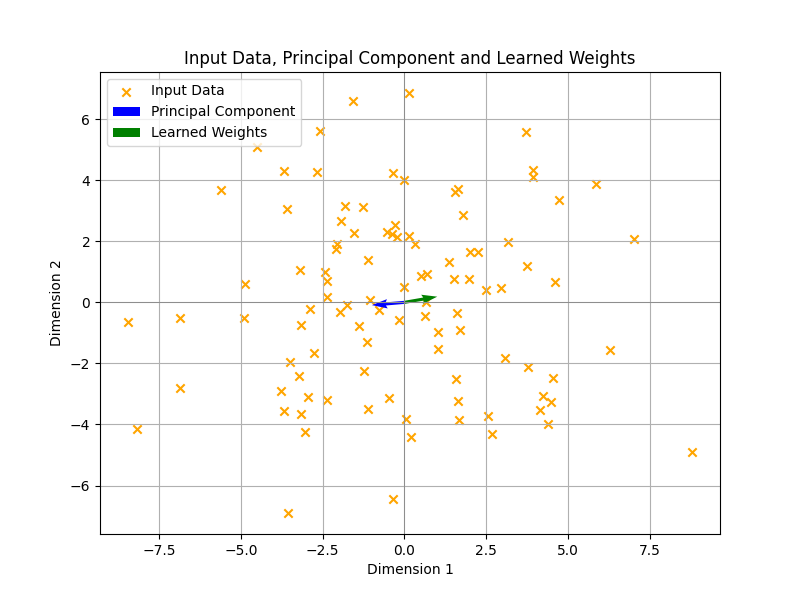
\includegraphics[width=0.75\textwidth]{oja_rule.png}
    \caption{Oja's Rule Converging to the First Principal Component of the Input Data}
    \label{fig:oja_rule}
\end{figure}

We can see that the learned weight vector and the first principal component are roughly on the same line but pointing in opposite directions. Since eigenvectors are direction invariant, we can flip either the learned weight vector or the first principal component and they will be exactly the same. This demonstrates empirically that Oja's rule converges to the first principal component of the input data.


\subsection{Causality detection in STDP}

STDP weight updates are based on the relative timing of the pre-synaptic and post-synaptic spikes. If the pre-synaptic spike occurs before the post-synaptic spike, the weight is increased and if the post-synaptic spike occurs before the pre-synaptic spike, the weight is decreased. This is based on the idea that the pre-synaptic neuron is the cause of the post-synaptic neuron firing. Below we show the mathematical formulation of the STDP weight update rule based on the relative timing of the pre-synaptic and post-synaptic spikes.

\begin{equation}
\Delta W =
\begin{cases}
    A_+ e^{\frac{t_{\text{pre}} - t_{\text{post}}}{\tau_+}}, & \text{if } t_{\text{post}} > t_{\text{pre}} \\
    -A_- e^{-\frac{t_{\text{pre}} - t_{\text{post}}}{\tau_-}}, & \text{if } t_{\text{post}} < t_{\text{pre}}
\end{cases}
\end{equation}

The following figure gives an empirical demonstration of the STDP weight update rule based on an example with two pre-synaptic neurons $A$ and $B$ and one post-synaptic neuron. The pre-synaptic neuron $B$ fires after the post-synaptic neuron and the pre-synaptic neuron $A$ fires before the post-synaptic neuron. We can see that the weight from neuron $A$ to the post-synaptic neuron is increased and the weight from neuron $B$ to the post-synaptic neuron is decreased. 

\begin{figure}[H]
    \centering
    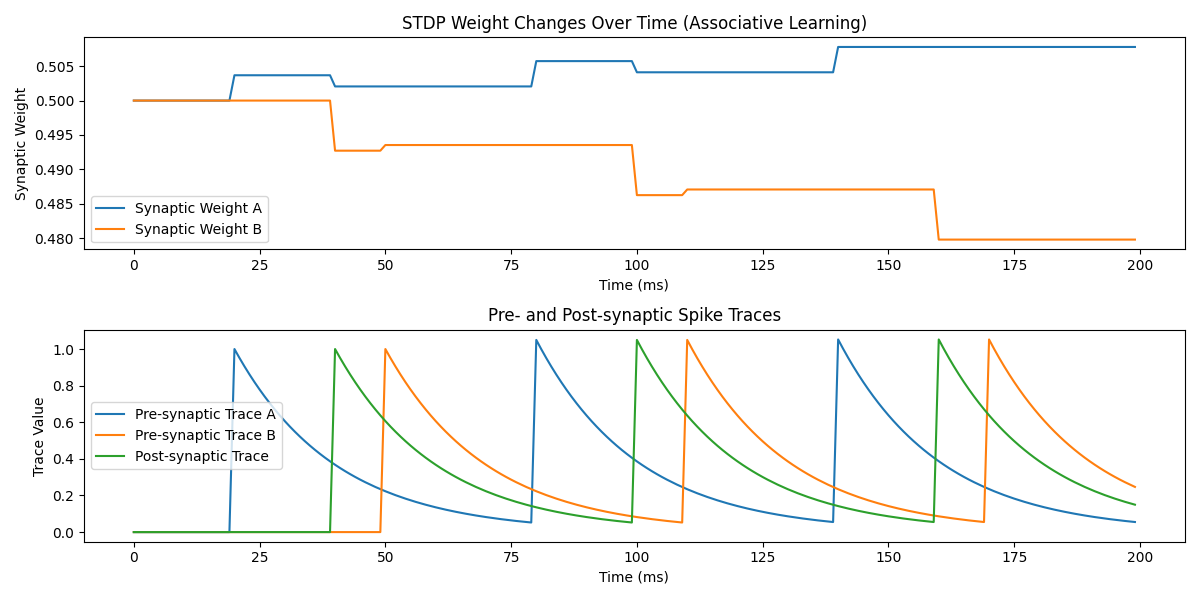
\includegraphics[width=0.75\textwidth]{stdp.png}
    \caption{STDP Weight Updates Based on Timing of Pre-synaptic and Post-synaptic Spikes}
    \label{fig:stdp}
\end{figure}


\subsection{Assessing the variance and bias of the learning algorithms}

\subsubsection{Empirical demonstration of variances of weight perturbation, node perturbation, and backpropagation using Signal-to-Noise Ratio}
We can assess the performance of different learning algorithms such as weight perturbation, node perturbation, and backpropagation by comparing the Signal-to-Noise Ratio (SNR) of gradients with backpropagation. The SNR is defined as the ratio of the mean of the output to the standard deviation of the output. A higher standard deviation relative to the mean indicates that there is much more noise in the gradients. Consequently, we would need more samples to achieve the same learning effectiveness. Below we show the empirical demonstration of the SNR of the gradients for weight perturbation, node perturbation, and backpropagation on the MNIST dataset.

\begin{figure}[H]
    \centering
    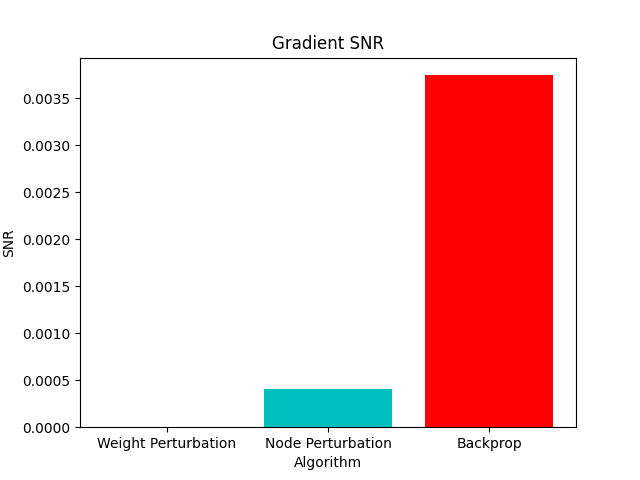
\includegraphics[width=.7\textwidth]{gradient_snr.png}
    \caption{Signal-to-Noise Ratio of Gradients for Weight Perturbation, Node Perturbation, and Backpropagation}
    \label{fig:gradient_snr}
\end{figure}

We can see that the SNR of the gradients for backpropagation is much higher than the SNR of the gradients for weight perturbation and node perturbation. The SNR for node perturbation appears to be slightly higher than the SNR for weight perturbation but both are significantly lower than the SNR for backpropagation.


\subsubsection{Cosine Similarity between backpropagation, feedback alignment, and Kolen-Pollack}

To assess the similarity between gradient updates for backpropagation, feedback alignment, and Kolen-Pollack, we can compute the cosine similarity between the gradients. The cosine similarity is defined as $C Sim(\Delta \theta_1, \Delta \theta_2) = \frac{\Delta \theta_1^T \Delta \theta_2}{\|\Delta \theta_1\|_2 \|\Delta \theta_2\|_2}$ where $\theta_1$ and $\theta_2$ are parameters in two different networks. In our case we are interested in comparing each of the networks with backpropagation and we expect that trivially backpropagation and itself will have a cosine similarity of 1. Below we show the empirical demonstration on the MNIST dataset of the cosine similarity between gradient updates for backpropagation, feedback alignment, and Kolen-Pollack on the hidden layer weights over 4 epochs.

\begin{figure}[H]
    \centering
    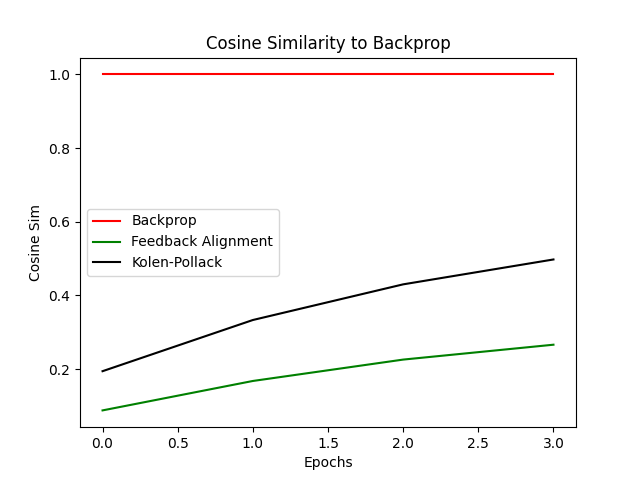
\includegraphics[width=.7\textwidth]{cosine_similarity.png}
    \caption{Cosine Similarity between Gradient Updates for Backpropagation, Feedback Alignment, and Kolen-Pollack}
    \label{fig:cosine_similarity}
\end{figure}

As expected, the cosine similarity between backpropagation and itself is 1. The cosine similarity between backpropagation and Kolen-Pollack is around 0.5 at the last epoch and the cosine similarity between backpropagation and Feedback Alignment is around 0.2. The random matrix $\mathbf{B}$ in Feedback Alignment is the cause of the lower cosine similarity with backpropagation since we can imagine it as a noisy version of $\mathbf{W^T}$. One potential reason why the cosine similarity between Kolen-Pollack and backpropagation is higher than the cosine similarity between Feedback Alignment and backpropagation is because Kolen-Pollack algorithm will update the matrix $\mathbf{B}$ to converge to $\mathbf{W_{\text{out}}^T}$. We can see that despite $\mathbf{B}$ converging only to $\mathbf{W_{\text{out}}^T}$, the cosine similarity between Kolen-Pollack and backpropagation for $\mathbf{W_{\text{hidden}}^T}$ is still much higher than Feedback Alignment.

\subsection{Randomness of matrix $\mathbf{B}$ in Feedback Alignment}

We can further explore how the values for the initialized random matrix $\mathbf{B}$ in Feedback Alignment affect the performance of the algorithm. To perform this comparison we can look into 5 different random seeds for the matrix $\mathbf{B}$ and compare the loss and accuracy of the Feedback Alignment algorithm on the MNIST dataset. Below we show the performance results of Feedback Alignment on the MNIST dataset with 5 different random seeds used to initialize the matrix $\mathbf{B}$.

\begin{figure}[H]
    \centering
    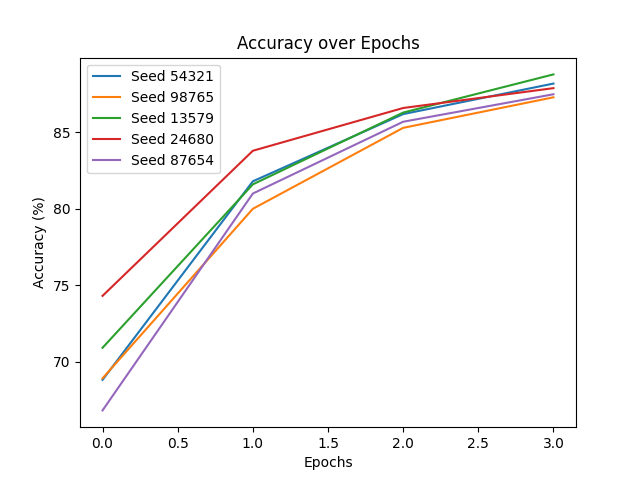
\includegraphics[width=.7\textwidth]{feedback_alignment_vary_B_accuracy.png}
    \caption{Feedback Alignment accuracy on MNIST with 5 Different Random Seeds}
    \label{fig:feedback_alignment_vary_B_accuracy}
\end{figure}

\begin{figure}[H]
    \centering
    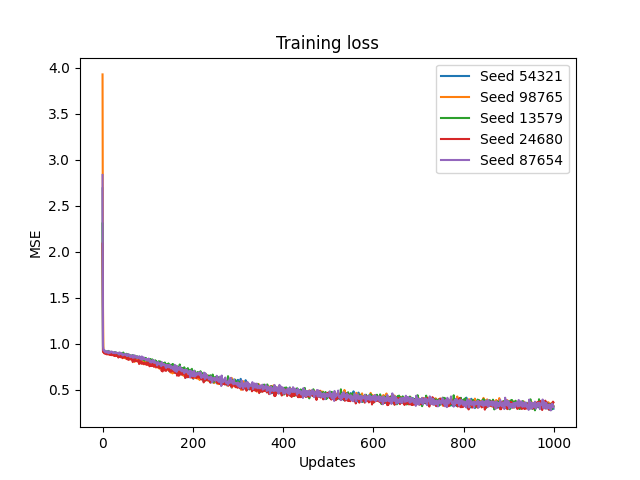
\includegraphics[width=.7\textwidth]{feedback_alignment_vary_B_loss.png}
    \caption{Feedback Alignment loss on MNIST with 5 Different Random Seeds}
    \label{fig:feedback_alignment_vary_B_loss}
\end{figure}

While there are some performance discrepancies in terms of accuracy, overall, the random initialization of the matrix $\mathbf{B}$ in Feedback Alignment does not seem to have a significant impact on the performance of the Feedback Alignment algorithm. The loss and accuracy of the algorithm are relatively consistent across the 5 different random seeds. This suggests that at least for a toy example like MNIST any approximation for $\mathbf{W^T}$ will be able to converge to a minimum close to backpropagation. 

\end{document}